\begin{center}
\Large\textbf{BIOGRAFI PENULIS}
\end{center}
\vspace{1ex}

\begin{wrapfigure}{L}{0.3\textwidth}
	\centering
	\vspace{-3ex}	
	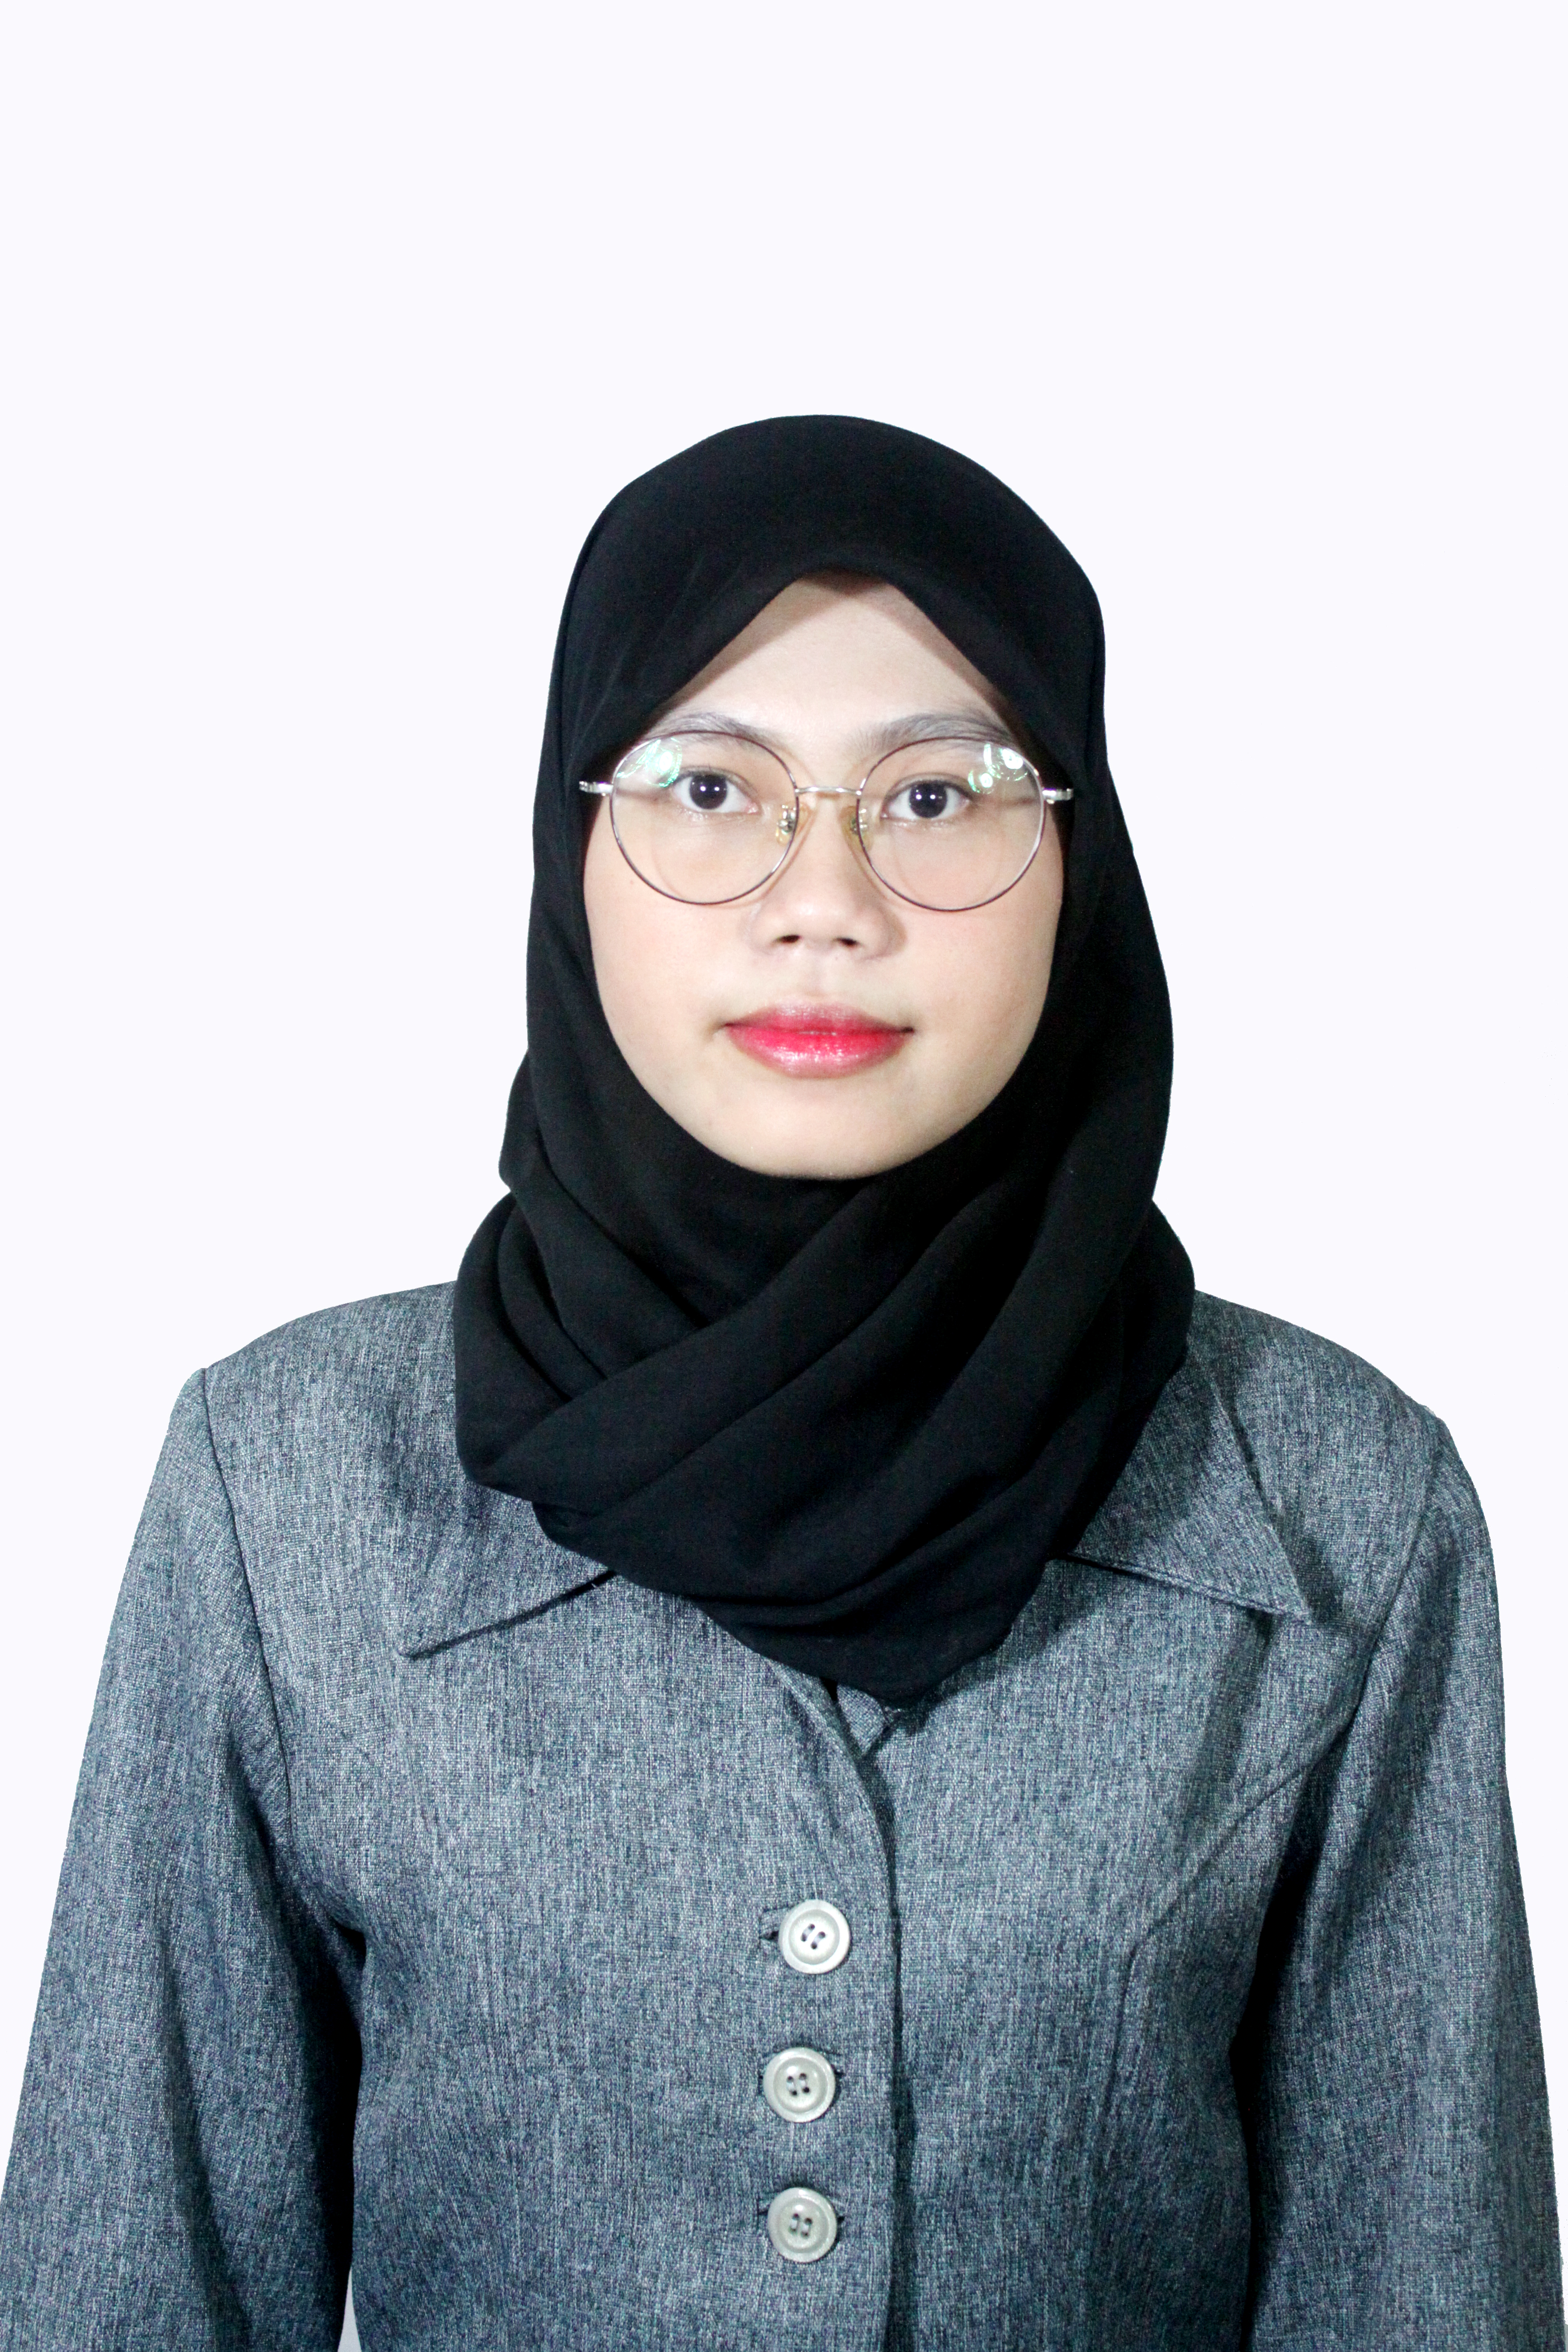
\includegraphics[width=3cm]{img/lampiran/fotoformal.jpg}
	\vspace{-4ex}
\end{wrapfigure}
\noindent 
Fernanda Daymara Hasna, atau yang lebih akrab dipanggil Nanda, lahir di Magelang pada 21 Agustus 1998. Anak pertama dari tiga bersaudara ini telah menyelesaikan pendidikan di SMA Negeri 5 Kota Bekasi pada 2016 dan melanjutkannya di Departemen Teknik Komputer FTEIC-ITS. Selama menjadi mahasiswi ITS, penulis tertarik dengan bidang teknologi digital khususnya bidang \textit{IT Project Management}, \textit{User Oriented Product Development}, dan \textit{Design System Analysis}. Selain itu penulis juga aktif di bidang pengembangan diri melalui pelatihan keterampilan manajemen mahasiswa tingkat pra-dasar hingga menengah, kemudian diimplementasikan dalam organisasi UKM Robotika ITS dan berbagai kegiatan seperti \textit{Multimedia \& Game Event 2018}, ITS Expo 2017, dan lainnya.